
In the last four Chapters we have introduced seven important \PETSc types (object classes).  All are important for solving PDEs:

\medskip
\begin{tabular}{ll}
Chapter \ref{chap:ls}: \pVec, \pMat, \pKSP, \pPC \hspace{.5in} & for linear algebra \\
Chapter \ref{chap:st}: \pDMDA                    & for structured grids \\
Chapter \ref{chap:nl}: \pSNES                    & for Newton's method \\
Chapter \ref{chap:ts}: \pTS                      & for time-stepping
\end{tabular}

\bigskip

The structured-grid, steady-state examples in this and later Chapters will use the first six of these objects (Figure \ref{fig:of:standardstack}).  Unstructured-grid examples in Chapters \ref{chap:un} and \ref{chap:dp} will replace the \pDMDA mesh-topology object with naive and advanced (\pDMPlex) substitutes, respectively.

In other words, from now on we will even solve \emph{linear} PDEs using a nonlinear-solver \pSNES object.  Examples are in Chapters \ref{chap:un} and \ref{chap:ad}.  In such cases we know that one Newton iteration suffices in theory.  Always using \pSNES allows uniform code structure and more flexibility when it comes to changing the PDE problem.

Though new ideas appear here, the current Chapter takes a break from introducing new \PETSc types.  Instead we look at a PDE which arises from minimization in a function space, and we introduce a structured-grid finite element method.  This example is a nonlinear Poisson-like equation with solution-dependent diffusivity.

\begin{figure}
% usage: \standardSNESstack{scale}{objective}{Jacobian}{DMDA}
\standardSNESstack{0.9}{}{dashed}{}
\caption{The ``\PETSc stack'' for \pSNES- and \pDMDA-based examples which solve a PDE arising from minimization of an objective function.  Compare Figures \ref{fig:st:linearstack} and \ref{fig:nl:reactionstack}.}
\label{fig:of:standardstack}
\end{figure}

Figure \ref{fig:of:standardstack} shows the ``stack'' of \PETSc components for solving PDEs which arise from optimization problems.  Initial implementations require user code for an objective function and/or a residual function---otherwise \PETSc has \emph{no} description of your problem---but Jacobians are also often implemented.

The example code in the current Chapter is the last one shown in full.  In later Chapters we show snippets.  The reader can always examine and run the complete codes by looking in the \texttt{c/} directory of the \texttt{p4pdes} repository.


\section{$p$-Laplacian equation as minimization}

Let $\Omega$ be a domain (connected open subset) in $\RR^2$ with well-behaved boundary.\sidenote{A Lipschitz boundary will suffice in theory.  In practice we use polygonal domains, namely a rectangle in the current Chapter and general polygons in Chapter \ref{chap:un}.}  For simplicity, noting our numerical method will use the point values of this function, suppose $f\in C(\overline \Omega)$ is given.  Consider this nonlinear functional for $p \ge 1$,
\begin{equation}
    I[u] = \int_\Omega \frac{1}{p} |\grad u|^p - fu.  \label{eq:of:functional}
\end{equation}
This functional is well-defined and continuous on the Sobolev space \citep{AdamsFournier2003,Evans2010} of integrable functions on $\Omega$ which have integrable gradient,
\begin{equation}
    W^{1,p}(\Omega) = \left\{w \,:\, \int_\Omega |w|^p < \infty \,\, \& \, \int_\Omega |\grad w|^p < \infty\right\}, \label{eq:of:sobolevdefn}
\end{equation}
a Banach space with norm $\|w\|_{W^{1,p}} = \left(\int_\Omega |w|^p + \int_\Omega |\grad w|^p\right)^{1/p}$.

\begin{marginfigure}
\includegraphics[width=1.2\textwidth]{figs/minsurf} % generated by figs/minsurf.tex
\medskip
\caption{The functional $I[u]$ is analogous to the convex surface $z = \tfrac{1}{4}(x^4 + y^4) - 2x + 2y$ shown here, but with input from the $\infty$-dimensional space $W_g^{1,p}(\Omega)$ instead of the plane $\RR^2$.}
\label{fig:of:cartoonfunctional}
\end{marginfigure}

The reader may visualize $I[u]$ in cartoon form as in Figure \ref{fig:of:cartoonfunctional}.  As suggested by the cartoon, this functional has a unique minimum, at least once we add boundary conditions.

We add Dirichlet conditions (Chapter \ref{chap:st}) by choosing a real-valued function $g$, defined along $\partial \Omega$, so as to determine an affine subspace of $W^{1,p}(\Omega)$, namely
\begin{equation}
    W_g^{1,p}(\Omega) = \left\{w \,:\, w \in W^{1,p}(\Omega) \,\, \& \,\, w\big|_{\partial \Omega} = g\right\}.  \label{eq:of:affinedirichlet}
\end{equation}
For this to make sense one might require $g \in L^p(\partial \Omega)$ and note that the equation $w\big|_{\partial \Omega} = g$ has a precise ``trace operator'' meaning \citep[section 5.5]{Evans2010}.  Again, however, because our numerical scheme will use the point values of $g$, we assume $g\in C(\partial\Omega)$.  These considerations also define a vector subspace $W_0^{1,p}(\Omega) \subset W^{1,p}(\Omega)$, in the case where $g=0$, which we will use for ``test'' functions below.

The functional $I[u]$ has two significant properties.  First, $I[u]$ is \emph{coercive} in the sense that if the input function is large in norm then the output is large:
\begin{equation}
\lim_{\|u\|_{W^{1,p}} \to +\infty} I[u] = +\infty.   \label{eq:of:coercivity}
\end{equation}
Second it is \emph{convex}, meaning that
\begin{equation}
I[\lambda u + (1-\lambda) v] \le \lambda I[u] + (1-\lambda) I[v]    \label{eq:of:convexity}
\end{equation}
if $u,v\in W_g^{1,p}(\Omega)$ and $0 \le \lambda \le 1$.  We say $I[u]$ is \emph{strictly convex} if $\|u-v\|_{W^{1,p}} > 0$ and $0 < \lambda < 1$ implies strict inequality in \eqref{eq:of:convexity}.  These two properties of $I[u]$, coercivity and convexity, are addressed in Exercise \ref{chap:of}.\ref{exer:of:twoproperties}.

A standard theorem in the calculus of variations \citep[Theorem 8.2.2]{Evans2010} shows that the coercivity and strict convexity of $I[u]$ suffice to imply that the problem
\begin{equation}
\min_{u \in W_g^{1,p}(\Omega)} I[u] \label{eq:of:plapmin}
\end{equation}
has a unique solution.  Strict convexity is used to show uniqueness, but convexity also implies that $I[u]$ is continuous enough to have a minimum on compact sets in the appropriate topology.\sidenote{Namely $I[u]$ is \emph{weakly lower semi-continuous}. This means, by definition, that $\liminf_{v\rightharpoonup u} I[v] \ge I[u]$, using the weak topology on $W^{1,p}(\Omega)$ \citep[section 8.2]{Evans2010}.}  Compactness arises from coercivity in the sense that bounded, closed subsets of $W^{1,p}(\Omega)$, which arise in the existence proof as sets $\{w\,:\,I[w] \le L\}$, are compact in the weak topology.

Being good calculus students we seek the solution to minimization problem \eqref{eq:of:plapmin} by taking the derivative (gradient) and setting it to zero.  If $p>1$ then the functional $I[u]$ is smooth enough to have a gradient, as we show next.  The solution of minimization \eqref{eq:of:plapmin} is then also the solution to a nonlinear equation.

Assume $\eps\in \RR$ and $u,v \in W^{1,p}(\Omega)$.  Then, by the binomial theorem,
\begin{align*}
I[u+\eps v] - I[u] &= \int_\Omega \frac{1}{p} |\grad u + \eps \grad v|^p - \frac{1}{p} |\grad u|^p - \eps f v \\
   &= \eps \left(\int_\Omega |\grad u|^{p-2} \grad u \cdot \grad v - f v\right) + O(\eps^2).
\end{align*}
Thus the directional derivative exists and has this formula:
\begin{equation}
\grad I[u](v) = \lim_{\eps\to 0} \frac{I[u+\eps v] - I[u]}{\eps} = \int_\Omega |\grad u|^{p-2} \grad u \cdot \grad v - f v. \label{eq:of:plapfunctionalderivative}
\end{equation}
That is, for each $u \in W^{1,p}(\Omega)$, formula \eqref{eq:of:plapfunctionalderivative} defines a linear and continuous map, the gradient
   $$\grad I[u] : W^{1,p}(\Omega) \to \RR.$$

If $u \in W_g^{1,p}(\Omega)$ and $v\in W_0^{1,p}(\Omega)$ then $u+\eps v\in W_g^{1,p}(\Omega)$.  Thus if $u \in W_g^{1,p}(\Omega)$ solves \eqref{eq:of:plapmin} then the above calculation also shows $\grad I[u](v)=0$ or
\begin{equation}
\int_\Omega |\grad u|^{p-2} \grad u \cdot \grad v - f v = 0 \label{eq:of:plapweakform}
\end{equation}
for all $v\in W_0^{1,p}(\Omega)$.  Note that the test functions $v$ have zero boundary values in this calculation.  We refer to \eqref{eq:of:plapweakform} as the \emph{weak form} of the $p$-\emph{Laplacian} equation.\sidenote{Alternate names include \emph{variational equation} and \emph{Euler-Lagrange equation}.}

If the solution $u \in W_g^{1,p}(\Omega)$ to problem \eqref{eq:of:plapmin} or equation \eqref{eq:of:plapweakform} is actually smooth enough to have continuous second derivatives\sidenote{\emph{Proving} this much smoothness is possible in some cases when the domain $\Omega$ and data $f,g$ are well-behaved, but beyond our scope.} then we can derive the \emph{strong form} PDE \eqref{eq:of:plapstrongform} below, as follows.  An integration-by-parts \citep[Appendix C]{Evans2010} gives
    $$-\int_\Omega \Div\left(|\grad u|^{p-2} \grad u\right) v - \int_\Omega f v + \int_{\partial \Omega} v |\grad u|^{p-2} \grad u \cdot \bn = 0.$$
The boundary integral is zero because $v\in W_0^{1,p}(\Omega)$.  It follows that
\begin{equation}
- \Div\left(|\grad u|^{p-2} \grad u\right) = f.
\label{eq:of:plapstrongform}
\end{equation}
This is the traditional form of the $p$-Laplacian equation, and it reduces to the Poisson equation \eqref{poissonsquare} if $p=2$.

Before proceeding to a numerical solution, the main ideas of the above theory are simple and worth restating:
\begin{quote}
Minimization problem \eqref{eq:of:plapmin} is equivalent to the weak form \eqref{eq:of:plapweakform}.  These become the strong form \eqref{eq:of:plapstrongform} when the solution $u$ is smooth.  Thus the $p$-Laplacian equation arises from minimization.
\end{quote}

We pause to choose a particular test problem for which the exact solution is known.  An easy choice is to ``manufacture'' a test problem by starting with a simple solution with one parameter $\alpha\in\RR$:
\begin{equation}
    u_{\text{exact}}(x,y) = \frac{1}{2} (x+\alpha)^2 (y+\alpha)^2. \label{eq:of:exactsolution}
\end{equation}
This formula also determines $g$ along $\partial \Omega$.  The source function $f$ is then computed by-hand from the strong form \eqref{eq:of:plapstrongform}.  (This calculation is error-prone, too, but by-hand errors are not correlated to code implementation errors.  Agreement is likely to reflect correctness.)

If $\alpha>0$ then the coefficient of the $p$-Laplacian equation, namely $|\grad u|^{p-2}$, is bounded below by a positive constant, and that it is bounded above.  Thus equation \eqref{eq:of:plapweakform}, or \eqref{eq:of:plapstrongform}, is uniformly elliptic \citep{Evans2010} at the solution \eqref{eq:of:exactsolution}.  However, though such bounds apply at the solution $u=u_{\text{exact}}$, they do not necessarily apply to the approximations (iterates) in a numerical procedure, so the iteration might ``lose ellipticity'' on the way to the solution.  We will return to such considerations, and consider the $\alpha \le 0$ cases and the corresponding need for regularization, once we have an implementation.


\section{Structured $Q^1$ finite elements}

Initially we will use \PETSc to numerically solve the $p$-Laplacian equation as minimization problem \eqref{eq:of:plapmin}, based only on code that computes the functional $I[u]$ from a representation of $u \in W_g^{1,p}(\Omega)$.  Thus, once we have a finite-dimensional representation of the input $u$, we need only implement formula \eqref{eq:of:functional} for $I[u]$.

Such a minimization approach may suffice for prototyping, but we will augment it by additional derivative-computing code so that the problem becomes a nonlinear-residual problem like that of Chapter \ref{chap:nl}.  Initially, however, we will ask \PETSc to use finite differences when it needs derivatives (gradients) in minimizing $I[u]$.  In this case the nonlinear equations, and the associated residual functions, are approximate and are internal to \PETSc.

For the representation of $u$ we introduce a structured-grid finite element method (FEM) using quadrilateral elements.  The gridded unknowns, which live on a structured grid somewhat different from that in Chapter \ref{chap:st}, now represent an element of a function space.

\begin{figure}
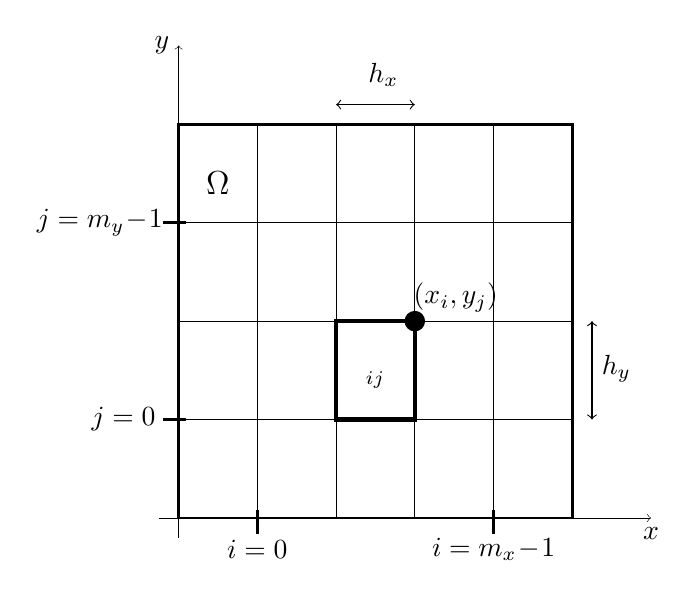
\begin{tikzpicture}[scale=5.0]
  % axes
  \draw[->,very thin] (-0.05,0.0) -- (1.2,0.0) node[below] {$x$};
  \draw[->,very thin] (0.0,-0.05) -- (0.0,1.2) node[left] {$y$};
  % grid
  \draw[line width=1.0pt] (0.0,0.0) -- (0.0,1.0) -- (1.0,1.0) -- (1.0,0.0) -- cycle;
  \pgfmathsetmacro\fifth{1.0/5.0}
  \pgfmathsetmacro\fourth{1.0/4.0}
  \draw[xstep=\fifth,ystep=\fourth,black,thin] (0.0,0.0) grid (1.0,1.0);
  \node at (0.1,0.85) {\large $\Omega$};
  % outline an element, showing location and dimensions
  \draw[line width=1.5pt] (0.6,0.5) -- (0.4,0.5) -- (0.4,0.25) -- (0.6,0.25) -- cycle;
  \node at (0.5,0.35) {$\square_{ij}$};
  \filldraw (0.6,0.5) circle (0.7pt) node[xshift=5.2mm,yshift=3mm] {$(x_i,y_j)$};
  \draw[<->] (0.4,1.05) -- (0.6,1.05) node[above,yshift=1mm,xshift=-4mm] {$h_x$};
  \draw[<->] (1.05,0.25) -- (1.05,0.5) node[right,yshift=-6mm] {$h_y$};
  % tick marks for i
  \draw[line width=1.0pt] (0.2,-0.04) -- (0.2,0.02);
  \draw[line width=1.0pt] (0.8,-0.04) -- (0.8,0.02);
  \node[yshift=-4mm] at (0.2,0.0) {$i=0$};
  \node[yshift=-4mm] at (0.8,0.0) {$i=m_x\!-\!1$};
  % tick marks for j
  \draw[line width=1.0pt] (-0.04,0.25) -- (0.02,0.25);
  \draw[line width=1.0pt] (-0.04,0.75) -- (0.02,0.75);
  \node[xshift=-7mm] at (0.0,0.25) {$j=0$};
  \node[xshift=-10mm] at (0.0,0.75) {$j=m_y\!-\!1$};
\end{tikzpicture}


\caption{The structured grid divides the unit square $\Omega$ into elements $\square_{ij}$ of area $h_x h_y$.  There are $N=m_x m_y$ interior nodes (degrees of freedom).  We index elements by their upper-right corners.}
\label{fig:of:q1grid}
\end{figure}

For this Chapter let $\Omega$ be the square $(0,1)\times (0,1)$.  Consider the structured grid on $\Omega$ shown in Figure \ref{fig:of:q1grid}.  Let $m_x,m_y$ be positive integers and define $h_x = 1/(m_x+1)$ and $h_y = 1/(m_y+1)$.  The structured grid is
\begin{equation}
x_i = (i+1) h_x, \qquad y_j = (j+1) h_y \label{eq:of:structuredgridindexing}
\end{equation}
for $i=-1,0,\dots,m_x$ and $j=-1,0,\dots,m_y$, giving $\tilde N = (m_x+2)(m_y+2)$ total nodes in the grid.  The $N=m_x\, m_y$ interior nodes are points with $0 \le i \le m_x-1$ and $0 \le j \le m_y-1$.  These interior nodes correspond to the degrees of freedom; the boundary values of $u\in W_g^{1,p}(\Omega)$ come from $g$. 

The grid has $(m_x+1)(m_x+1)$ rectangular \emph{elements}
   $$\square_{ij} = [x_{i-1},x_i] \times [y_{j-1},y_j]$$
for $i=0,\dots,m_x$ and $j=0,\dots,m_y$.  We index the elements by their upper-right corners.

The functional in \eqref{eq:of:functional} can be computed element-by-element,\footnote{Because element boundaries have zero measure and integration is additive.}
\begin{equation}
I[u] = \sum_{i=0}^{m_x} \sum_{j=0}^{m_y} \int_{\square_{ij}} \frac{1}{p} |\grad u|^p - fu  \label{eq:of:sumoverelements}
\end{equation}
Integration over a single element $\square_{ij}$ can be addressed once we represent $f$ and $u$.  A related sum over elements computes an approximation of the weak form \eqref{eq:of:plapweakform}; see \eqref{eq:of:weakformbasis} and \eqref{eq:of:weakformdetail} below.

By showing the grid in Figure \ref{fig:of:q1grid}, and the sum-over-elements formula \eqref{eq:of:sumoverelements}, we have already motivated how we are going to use \PETSc's \pDMDA structured-grid object.\sidenote{Introduced in Chapter \ref{chap:st}.}  We create this object using a \texttt{BOX} stencil and \texttt{GHOSTED} boundaries in each direction, as in this call extracted from Code \ref{code:plapMain}:
\begin{code}
  DMDACreate2d(COMM,
      DM_BOUNDARY_GHOSTED, DM_BOUNDARY_GHOSTED, DMDA_STENCIL_BOX,
      -3,-3,PETSC_DECIDE,PETSC_DECIDE,1,1,NULL,NULL,&da);
\end{code}
(Note we set the grid defaults to $m_x=m_y=3$.)  Thus if we create a \pVec \texttt{v} using ``\texttt{DMCreateLocalVector(da,\&v)}'' then it can store values at all $\tilde N = (m_x+2)(m_y+2)$ grid points, with the boundary points in the ghosts, while a \texttt{Global} \pVec from \texttt{DMCreateGlobalVector()} can store the $N=m_x m_y$ degrees of freedom.

On the other hand, how should we approximate a function $w \in W^{1,p}(\Omega)$ in a manner compatible with a structured grid of rectangles?  One simple choice requires that the approximation $w_h$ be bilinear on each element $\square_{ij}$ and continuous on the whole domain $\Omega$.  These requirements determine $w_h(x,y)$ from the nodal values $w_{ij} = w_h(x_i,y_j)$.  Said another way, there is a linear isomorphism between the vector space $\RR^{\tilde N}$, and an $\tilde N$-dimensional linear subspace of $W^{1,p}(\Omega)$, namely
\begin{equation}
S^h = \left\{v \in C(\Omega) \, \Big| \, v|_{\square_{ij}} \text{ is bilinear}\right\}. \label{eq:of:Shdefn}
\end{equation}
Because the elements are quadrilaterals and the polynomial degree is one, $S^h$ is called a $Q^1$ \emph{finite element space} \citep{Elmanetal2005}

The solution $u$ to minimization problem \eqref{eq:of:plapmin} must, however, have the boundary values given by $g$.  We would want $g$ to be continuous and (appropriately) piece-wise linear on $\partial\Omega$, as otherwise its use conflicts with the restrictions which define $S^h$.  In that case, one may show that the functions
\begin{equation}
S_g^h = \left\{v \in S^h \, \Big| \, v|_{\partial \Omega} = g\right\} \label{eq:of:Sghdefn}
\end{equation}
form an (affine) subspace of $W_g^{1,p}(\Omega)$.  Replacing $W_g^{1,p}(\Omega)$ by $S_g^h$ in problem \eqref{eq:of:plapmin} is a \emph{conforming}\sidenote{A ``nonconforming'' version might have $u_h|_{\partial \Omega}$ as the piecewise-linear interpolant of $g$.} $Q^1$ FEM.  Because an element of $S_g^h$ is entirely determined by its values on interior nodes, $S_g^h$ is an $N=m_x m_y$ dimensional affine subspace of $S^h$.


\section{Formulas on one element}

The next step is to describe a bilinear function on a single element $\square_{ij}$, and to thereby build a basis for space $S_g^h$.  We do this by constructing bilinear functions on a \emph{reference element}
    $$\square_\ast = [-1,1]\times[-1,1]$$
in variables $\xi$ and $\eta$, as shown in Figure \ref{fig:of:q1gridandref}.\sidenote{One may easily avoid using the reference element because all elements are congruent rectangles.  We are, however, thinking ahead toward unstructured examples (Chapter \ref{chap:un}).}

If $v(\xi,\eta)$ is bilinear on $\square_\ast$ then $v(\xi,\eta) = a + b\, \xi + c\, \eta + d\, \xi \eta$.  The monomial basis $\{1,\xi,\eta,\xi\eta\}$ is not, however, a convenient one.  Instead, number the vertices (nodes) of $\square_\ast$ as shown in Figure \ref{fig:of:q1gridandref}:
\begin{align}
(\xi_0,\eta_0) &= (+1,+1), \quad (\xi_1,\eta_1) = (-1,+1),    \label{eq:of:refcorners} \\
(\xi_2,\eta_2) &= (-1,-1), \quad (\xi_3,\eta_3) = (+1,-1). \notag
\end{align}
The four functions
\begin{equation}
\chi_\ell(\xi,\eta) = \frac{1}{4} \left(1 + \xi_\ell \xi\right) \left(1 + \eta_\ell \eta\right)  \quad \text{ for } \ell=0,1,2,3 \label{eq:of:chidefn}
\end{equation}
form a basis of bilinear functions on $\square_\ast$.  The nodal values satisfy $\chi_\ell(\xi_{\ell'},\eta_{\ell'}) = \delta_{\ell\ell'}$ so expanding in this basis uses coefficients equal to the nodal values:
\begin{equation}
v(\xi,\eta) = \sum_{\ell=0}^3 v(\xi_\ell,\eta_\ell) \chi_\ell(\xi,\eta). \label{eq:of:bilinearrepresentationref}
\end{equation}

\begin{figure}
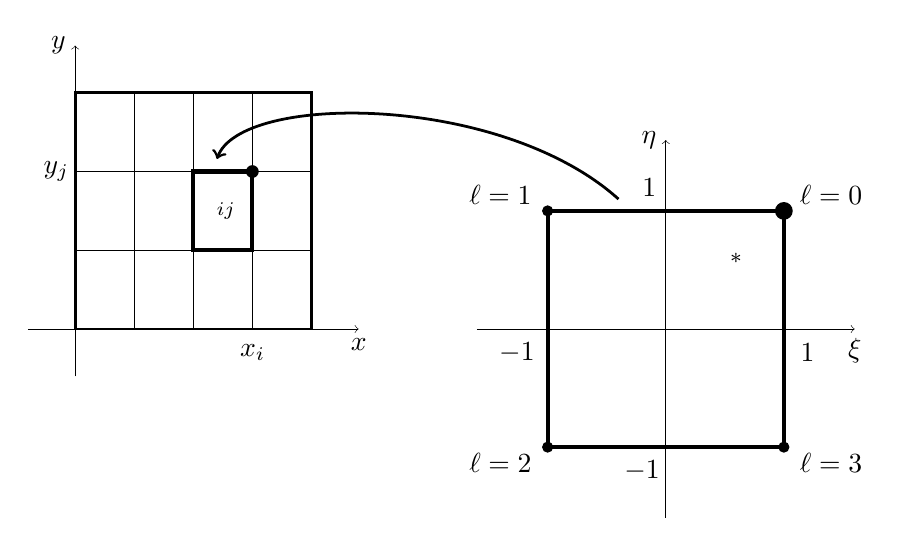
\begin{tikzpicture}[scale=3.0]
% (x,y) elements
  \draw[->,very thin] (-0.2,0.0) -- (1.2,0.0) node[below] {$x$};
  \draw[->,very thin] (0.0,-0.2) -- (0.0,1.2) node[left] {$y$};
  \draw[line width=1.0pt] (0.0,0.0) -- (0.0,1.0) -- (1.0,1.0) -- (1.0,0.0) -- cycle;
  \pgfmathsetmacro\fourth{1.0/4.0}
  \pgfmathsetmacro\third{1.0/3.0}
  \pgfmathsetmacro\twothird{2.0/3.0}
  \draw[xstep=\fourth,ystep=\third,black,thin] (0.0,0.0) grid (1.0,1.0);
  % outline an element
  \draw[line width=1.5pt] (0.5,\third) -- (0.75,\third) -- (0.75,\twothird) -- (0.5,\twothird) -- cycle;
  \node at (0.64,0.5) {$\square_{ij}$};
  \node at (0.751,-0.1) {$x_i$};
  \node at (-0.08,\twothird) {$y_j$};
  \filldraw (0.75,\twothird) circle (0.7pt);

% (xi,eta) reference element
% origin of axes at (2.5,0.0) and square has half-width 0.5
  \draw[->,very thin] (1.7,0.0) -- (3.3,0.0) node[below] {$\xi$};
  \draw[->,very thin] (2.5,-0.8) -- (2.5,0.8) node[left] {$\eta$};
  \draw[line width=1.5pt] (2.0,-0.5) -- (3.0,-0.5) -- (3.0,0.5) -- (2.0,0.5) -- cycle;
  \node at (3.1,-0.1) {$1$};
  \node at (1.87,-0.1) {$-1$};
  \node at (2.43,0.6) {$1$};
  \node at (2.4,-0.6) {$-1$};
  \node at (2.8,0.3) {\large $\square_\ast$};
  \filldraw (3.0,0.5) circle (1.0pt) node[xshift=6mm,yshift=2mm] {$\ell=0$};
  \filldraw (2.0,0.5) circle (0.6pt) node[xshift=-6mm,yshift=2mm] {$\ell=1$};
  \filldraw (2.0,-0.5) circle (0.6pt) node[xshift=-6mm,yshift=-2mm] {$\ell=2$};
  \filldraw (3.0,-0.5) circle (0.6pt) node[xshift=6mm,yshift=-2mm] {$\ell=3$};
% arc:
  \draw[->,line width=1.0pt] (2.3,0.55) .. controls (1.8,1.0) and (0.7,1.0) .. (0.6,0.72);
\end{tikzpicture}


\caption{Each element $\square_{ij}$ is the image under the map \eqref{eq:of:referencemap} from the reference element $\square_\ast$.  The corners of $\square_\ast$ are numbered $\ell=0,1,2,3$.  The $\ell=0$ corner maps to $(x_i,y_j)$.}
\label{fig:of:q1gridandref}
\end{figure}

The element map $\square_\ast \to \square_{ij}$ pictured in Figure \ref{fig:of:q1gridandref} can be written using the above basis functions $\chi_\ell$, or in simplified form:
\begin{align}
x(\xi,\eta) &= \sum_{\ell=0}^3 x_\ell \chi_\ell(\xi,\eta) = x_i + \frac{h_x}{2} (\xi-1), \label{eq:of:referencemap} \\
y(\xi,\eta) &= \sum_{\ell=0}^3 y_\ell \chi_\ell(\xi,\eta) = y_j + \frac{h_y}{2} (\eta-1). \notag
\end{align}
The Jacobian determinant of this map, used in integrals below, is the ratio of the area of $\square_{ij}$ to that of $\square_\ast$:
\begin{equation}
\left|\det\frac{\partial(x,y)}{\partial(\xi,\eta)}\right| = \det\begin{bmatrix} \frac{h_x}{2} & 0 \\ 0 & \frac{h_y}{2} \end{bmatrix} = \frac{h_x h_y}{4}. \label{eq:of:elementjacobian}
\end{equation}

For each node $(x_p,y_q)$ in the structured grid there is a continuous, piecewise-bilinear function $\psi_{p,q} \in S^h$, defined on all of $\overline\Omega$, which is equal to one on that node and equal to zero at all others:
\begin{equation}
  \psi_{p,q}(x_r,y_s) = \delta_{pr} \delta_{qs}.  \label{eq:of:psinodewise}
\end{equation}
Observe that $\psi_{p,q}$ is identically zero on every element which does not contain $(x_p,y_q)$.  Such ``hat'' functions, illustrated in Figure \ref{fig:of:q1hat}, form a basis of $S^h$.

\begin{marginfigure}
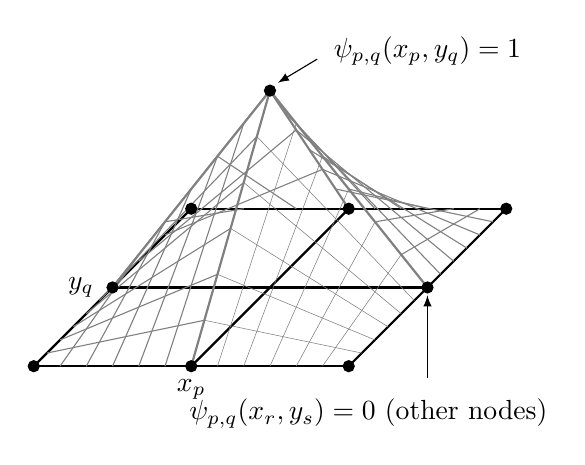
\begin{tikzpicture}[scale=0.5]

  % strong grid around elements
  \draw[thick] (0,0) -- (8,0);
  \draw[thick] (2,2) -- (10,2);
  \draw[thick] (4,4) -- (12,4);
  \draw[thick] (0,0) -- (4,4);
  \draw[thick] (4,0) -- (8,4);
  \draw[thick] (8,0) -- (12,4);

  \def\ytop{7};

  % tent lines
  \draw[gray,thick] (6,\ytop) -- (4,0);
  \draw[gray,thick] (6,\ytop) -- (2,2);
  \draw[gray,thick] (6,\ytop) -- (10,2);
  \draw[gray,thick] (6,\ytop) -- (8,4);

  \def\dx{(10.0-6.0)/6};
  \def\dy{(2.0-\ytop)/6};
  \foreach \jj in {1,...,5}
  {
       \draw[gray,very thin] ({6+\jj*\dx},{\ytop+\jj*\dy}) -- ({4+(4/6)*\jj},0.0);
  }

  \def\dx{(4.0-6.0)/6};
  \def\dy{(0.0-\ytop)/6};
  \foreach \jj in {1,...,5}
  {
       \draw[gray,very thin] ({6+\jj*\dx},{\ytop+\jj*\dy}) -- ({10-(2/6)*\jj},{2-(2/6)*\jj});
  }

  \def\dx{(2.0-6.0)/6};
  \def\dy{(2.0-\ytop)/6};
  \foreach \jj in {1,...,5}
  {
       \draw[gray,thin] ({6+\jj*\dx},{\ytop+\jj*\dy}) -- ({4-(4/6)*\jj},0.0);
  }

  \def\dx{(4.0-6.0)/6};
  \def\dy{(0.0-\ytop)/6};
  \foreach \jj in {1,...,5}
  {
       \draw[gray,thin] ({6+\jj*\dx},{\ytop+\jj*\dy}) -- ({2-(2/6)*\jj},{2-(2/6)*\jj});
  }

  \def\dx{(10.0-6.0)/6};
  \def\dy{(2.0-\ytop)/6};
  \foreach \jj in {1,...,5}
  {
       \draw[gray,thin] ({6+\jj*\dx},{\ytop+\jj*\dy}) -- ({8+(4/6)*\jj},4.0);
  }

  \def\dx{(8.0-6.0)/6};
  \def\dy{(4.0-\ytop)/6};
  \foreach \jj in {1,...,5}
  {
       \draw[gray,thin] ({6+\jj*\dx},{\ytop+\jj*\dy}) -- ({10+(2/6)*\jj},{2+(2/6)*\jj});
  }

  \def\dx{(2.0-6.0)/3};
  \def\dy{(2.0-\ytop)/3};
  \foreach \jj in {1,...,2}  % reduce clutter
  {
       \draw[gray,thin] ({6+\jj*\dx},{\ytop+\jj*\dy}) -- ({8-(4/3)*\jj},4.0);
  }

  \def\dx{(8.0-6.0)/3};
  \def\dy{(4.0-\ytop)/3};
  \foreach \jj in {1,...,2}
  {
       \draw[gray,thin] ({6+\jj*\dx},{\ytop+\jj*\dy}) -- ({2+(2/3)*\jj},{2+(2/3)*\jj});
  }

  % nodes in base plane
  \filldraw (0,0) circle (4pt);
  \filldraw (4,0) circle (4pt);
  \filldraw (8,0) circle (4pt);
  \filldraw (2,2) circle (4pt);
  %\filldraw (6,2) circle (4pt);   % (x_j,y_k) is at (6,2)
  \filldraw (10,2) circle (4pt);
  \filldraw (4,4) circle (4pt);
  \filldraw (8,4) circle (4pt);
  \filldraw (12,4) circle (4pt);

  % node at tent top
  \filldraw (6,\ytop) circle (4pt);

  % annotate
  \draw (10,\ytop+1.0) node {$\psi_{p,q}(x_p,y_q)=1$};
  \draw[-latex] (7.2,\ytop+0.8) -- (6.2,\ytop+0.2);
  \draw (8.5,-1.2) node {$\psi_{p,q}(x_r,y_s)=0$ (other nodes)};
  \draw[-latex] (10,-0.3) -- (10,1.8);

  % label center point
  \draw (4,-0.6) node {$x_p$};
  \draw (1.2,2) node {$y_q$};

\end{tikzpicture}

\caption{A hat function $\psi_{p,q} \in S^h$.}
\label{fig:of:q1hat}
\end{marginfigure}

When restricted to a particular element $\square_{ij}$, and then pulled-back to the reference element $\square_\ast$, the hat function $\psi_{p,q}$ is either identically zero or it is equal to one of the basis functions $\chi_\ell$.  That is, if corner $(\xi_\ell,\eta_\ell) \in \square_\ast$ corresponds to node $(x_p,y_q) \in \overline\Omega$, under the element map onto $\square_{ij}$, then
\begin{equation}
  \psi_{p,q}(x(\xi,\eta),y(\xi,\eta)) = \chi_\ell(\xi,\eta).  \label{eq:of:psionref}
\end{equation}
However, to evaluate $I[u]$ in \eqref{eq:of:sumoverelements} we will also want to compute gradients in the original $(x,y)$ variables:
\begin{equation}
  (\grad_{x,y} \psi_{p,q})(x(\xi,\eta),y(\xi,\eta)) = \left<\frac{2}{h_x}\frac{\partial\chi_\ell}{\partial \xi},\frac{2}{h_y}\frac{\partial\chi_\ell}{\partial \eta}\right>.   \label{eq:of:gradpsionref}
\end{equation}
Derivatives $\partial\chi_\ell/\partial \xi$ and $\partial\chi_\ell/\partial \eta$ can be found from formula \eqref{eq:of:chidefn} above.  Checking equation \eqref{eq:of:gradpsionref} is an easy exercise.

Suppose we have $v \in S_0^h$; note that $S_0^h$ refers to the space defined by \eqref{eq:of:Sghdefn} where $g=0$ identically.  It can be represented using hat functions at the $N$ interior nodes
\begin{equation}
v(x,y) = \sum_{i=0}^{m_x-1} \sum_{j=0}^{m_y-1} v_{i,j} \psi_{i,j}(x,y) \label{eq:of:bilinearrepresentation}
\end{equation}
on $\Omega$.

On the other hand, suppose we have $v \in S^h$ with other boundary values.  It can be written almost the same as \eqref{eq:of:bilinearrepresentation} but with expanded summation ranges of $i=-1,0,\dots,m_x$ and $j=-1,0,\dots,m_y$, respectively, including the hat functions along the boundary.  We will see that \PETSc makes it easy to represent any function in $S^h$ through ``ghost values'' off the edge of our grid of interior nodes.

A bilinear function on element $\square_{i,j}$ pulls-back to the reference element $\square_\ast$, using local node numbering, as
\begin{equation}
v(\xi,\eta) = \sum_{\ell=0}^3 v_\ell \chi_\ell(\xi,\eta)  \qquad \text{on } \,\square_\ast. \label{eq:of:bilinearref}
\end{equation}
The coefficient $v_\ell$ is equal to $v_{r,s} = v(x_r,y_s)$ for $(x_r,y_s)\in\square_{i,j}$ corresponding under the element map to $(\xi_\ell,\eta_\ell) \in \square_\ast$.  Also, by \eqref{eq:of:gradpsionref} the $(x,y)$ gradient has formula:
\begin{equation}
  (\grad_{x,y} v)(\xi,\eta) = \left<\frac{2}{h_x} \sum_{\ell=0}^3 v_\ell \frac{\partial\chi_\ell}{\partial \xi}, \frac{2}{h_y} \sum_{\ell=0}^3 v_\ell \frac{\partial\chi_\ell}{\partial \eta}\right>. \label{eq:of:gradrepref}
\end{equation}


\section{Quadrature}

We do not plan to exactly-compute the integrals in \eqref{eq:of:sumoverelements}.  For general $p$ it would be quite challenging to exactly-integrate the term ``$|\grad u|^p$.''  Instead we will use numerical integration, also known a \emph{quadrature}.

First, change-of-variables transfers the integral to the reference element: If $v(x,y)$ is any integrable function on element $\square_{i,j}$ then, using the element map and \eqref{eq:of:elementjacobian}, we have
\begin{equation}
\int_{\square_{ij}} v(x,y)\,dx\,dy = \frac{h_x h_y}{4} \int_{\square_\ast} v(\xi,\eta) \,d\xi\,d\eta \label{eq:of:changeofvars}
\end{equation}
where $v(\xi,\eta)=v(x(\xi,\eta),y(\xi,\eta))$.

Next, recall Gauss-Legendre quadrature on integrals in one dimension \citep{GreenbaumChartier2012}:
\begin{equation}
\int_{-1}^1 f(z)\,dz \approx \sum_{q=0}^{n-1} w_q f(z_q).  \label{eq:of:gauss}
\end{equation}
For degrees $n=1,2,3$, the quadrature \emph{nodes} $z_q$ and \emph{weights} $w_q$ for integration over the interval $[-1,1]$ are given in Table \ref{tab:of:gauss}.  The degree $n$ rule is exact for polynomials of degree $2n-1$ and less.

\begin{table}[h]
\vspace{0.1in}

\begin{tabular}{lll}
$n$\phantom{foobar} & nodes $z_q$\phantom{foo} & weights $w_q$ \\ \hline
$1$ & $0$ & $2$ \\
$2$ & $-\frac{1}{\sqrt{3}}, +\frac{1}{\sqrt{3}}$ & $1,1$ \\
$3$ & $-\sqrt{\frac{3}{5}}, 0, +\sqrt{\frac{3}{5}}$ & $\frac{5}{9}, \frac{8}{9}, \frac{5}{9}$ \\
\end{tabular}

\vspace{0.1in}
\caption{Nodes and weights for low-degree Gauss-Legendre quadrature rules, for integrals \eqref{eq:of:gauss}.} \label{tab:of:gauss}
\end{table}

Rule \eqref{eq:of:gauss} extends to a product formula for integrals over $\square_\ast$:
\begin{equation}
\int_{\square_\ast} v(\xi,\eta) \,d\xi\,d\eta \approx \sum_{r=0}^{n-1} \sum_{s=0}^{n-1} w_r w_s v(z_r,z_s).  \label{eq:of:tensorgauss}
\end{equation}
The $n=2,3$ cases are shown in Figure \ref{fig:of:gausstwod}, while the $n=1$ rule is simply the midpoint rule on $\square_\ast$.

Formulas \eqref{eq:of:bilinearref}, \eqref{eq:of:gradrepref}, \eqref{eq:of:changeofvars}, and \eqref{eq:of:tensorgauss} combine to give an easily-computed approximation of integral in \eqref{eq:of:sumoverelements}.  On the reference element we define
\begin{equation}
G_{ij}(\xi,\eta) = \left[\frac{1}{p} |\grad u|^p - fu\right]_{\square_\ast} \label{eq:of:integrandheuristic}
\end{equation}
using the nodal values of $u$ and $f$ on element $\square_{ij}$.  (The details are in Exercise \ref{chap:of}.\ref{exer:of:integrand}.)  Then formula \eqref{eq:of:sumoverelements} becomes
\begin{equation}
I^h[u] = \frac{h_x h_y}{4} \quad \underbrace{\sum_{i=0}^{m_x} \sum_{j=0}^{m_y}}_{\begin{smallmatrix} \text{sum} \\ \text{over} \\ \text{elements} \end{smallmatrix}} \quad \underbrace{\sum_{r=0}^{n-1} \sum_{s=0}^{n-1}}_{\begin{smallmatrix} \text{sum} \\ \text{over} \\ \text{quadrature points} \end{smallmatrix}} \, w_r w_s G_{ij}(z_r,z_s). \label{eq:of:quadraturesumoverelements}
\end{equation}
We now have enough detail for a prototype implementation.

\begin{figure}
\newcommand{\gausssanspts}{
  % (xi,eta) reference element is square with half-width 1
  \draw[->,very thin] (-1.2,0.0) -- (1.2,0.0) node[below] {\small $\xi$};
  \draw[->,very thin] (0.0,-1.2) -- (0.0,1.2) node[left] {\small $\eta$};
  \draw[line width=1.5pt] (1.0,1.0) -- (-1.0,1.0) -- (-1.0,-1.0) -- (1.0,-1.0) -- cycle;
}

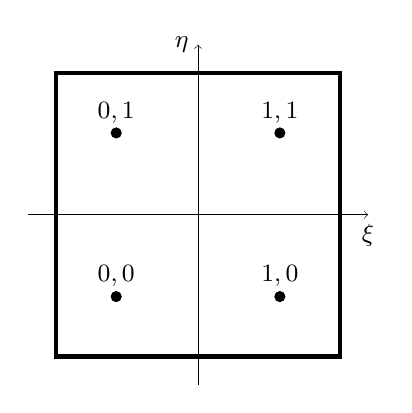
\begin{tikzpicture}[scale=1.8]
\gausssanspts
\pgfmathsetmacro\gl{1.0/sqrt(3.0)}
\foreach \x [count=\RR from 0] in {-\gl,\gl} {
    \foreach \y [count=\SS from 0] in {-\gl,\gl} {
         \filldraw (\x,\y) circle (1.0pt) node[above] {\small $\RR,\SS$};
    }
}
\end{tikzpicture}
\qquad\qquad
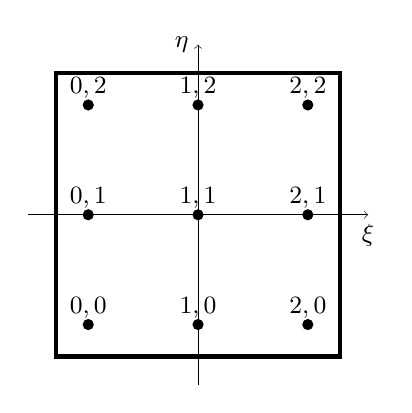
\begin{tikzpicture}[scale=1.8]
\gausssanspts
\pgfmathsetmacro\gl{sqrt(3.0/5.0)}
\foreach \x [count=\RR from 0] in {-\gl,0,\gl} {
    \foreach \y [count=\SS from 0] in {-\gl,0,\gl} {
         \filldraw (\x,\y) circle (1.0pt) node[above,yshift=-0.4mm] {\small $\RR,\SS$};
    }
}
\end{tikzpicture}


\caption{The $n=2$ (left) and $n=3$ (right) Gauss-Legendre quadrature points on the reference element $\square_\ast$.  Points $(z_r,z_s)$ are labeled as ``$r,s$''.  See equation \eqref{eq:of:tensorgauss} and Table \ref{tab:of:gauss}.}
\label{fig:of:gausstwod}
\end{figure}


\section{Objective-only implementation}

Our program \texttt{plap.c} is displayed in eight parts, Codes \ref{code:plapCtx}--\ref{code:plapFun}.  However, Code \ref{code:plapFun}, which implements the weak form \eqref{eq:of:plapweakform}, is shown after we get it running initially using only an implementation of objective functional \eqref{eq:of:functional}, that is, sum \eqref{eq:of:quadraturesumoverelements}.

\cinputpart{plap.c}{\CODELOC}{Declare and configure a context.}{I}{//STARTCTX}{//ENDCTX}{code:plapCtx}

Code \ref{code:plapCtx} declares a ``context'' \texttt{struct PLapCtx} which will be needed in the call-back functions \texttt{FormObjectiveLocal()} (Code \ref{code:plapObj}) and \texttt{FormFunctionLocal()} (Code \ref{code:plapFun}).  Defaults and \PETSc options are then set in the \texttt{ConfigureCtx()} function.  Note that exponent $p$ defaults to 4, the default for $\alpha$ in \eqref{eq:of:exactsolution} is 1, and the default for regularization parameter $\eps$ is zero.  (Until we explain how regularization could be used, starting on page \pageref{page:of:condellip}, we do not use it!)

\cinputpart{plap.c}{\CODELOC}{Set boundary values and initial iterate.  The boundary values set the ghosted nodes of a \texttt{Local} \pVec.}{II}{//STARTBDRYINIT}{//ENDBDRYINIT}{code:plapBI}

Next, in Code \ref{code:plapBI} we declare a function \texttt{BoundaryG()} for computing the boundary values $g(x,y)$.  (In fact this is just the exact solution $u(x,y)$ from \eqref{eq:of:exactsolution}.)  The function \texttt{SetGLocal()} sets boundary conditions at the ghosted points of the \texttt{Local} \pVec which stores $g$.  Also the function \texttt{InitialIterate()} sets the initial values of $u$ for the Newton iteration, by linearly-interpolating the boundary values into the interior nodes.

The third part, Code \ref{code:plapEx}, implements exact solution \eqref{eq:of:exactsolution} and computes the corresponding source term $f$ from PDE \eqref{eq:of:plapstrongform}.  In this case $f$ is computed at all grid points, including the ghost points of the \texttt{Local} \pVec which holds $f$, while the exact values of $u$ are only computed at the interior points; \texttt{uexact} is a \texttt{Global} \pVec.\sidenote{For ``fairness'' we will store the exact values of $u$ in a \pVec \texttt{uexact} which is unavailable to the call-back functions used in solving the PDE.}

A main concern in Codes \ref{code:plapBI} and \ref{code:plapEx} is that we will be able to integrate $u$, its derivatives, and $f$ on each element.  This requires ghosted values of $f$ and $g$.  These ghosted values are used in Codes \ref{code:plapTool}, \ref{code:plapObj}, and \ref{code:plapFun} below.

\cinputpart{plap.c}{\CODELOC}{Compute exact solution $u(x,y)$ from \eqref{eq:of:exactsolution}, and the corresponding source function $f(x,y)$.}{III}{//STARTEXACT}{//ENDEXACT}{code:plapEx}

We show FEM tools in Code \ref{code:plapFEM}.  These are generic to any $Q^1$ method in 2D which is based on a reference element.  We evaluate basis functions $\chi_\ell$, and their partial derivatives, at points $(\xi,\eta) \in \square_\ast$.  We also implement formulas \eqref{eq:of:chidefn}, \eqref{eq:of:bilinearref}, and \eqref{eq:of:gradrepref}.  Note that a two-element \texttt{struct gradRef} holds the components of a gradient at a point.  We also declare nodes and weights for degree $n=1,2,3$ Gauss-Legendre quadrature, with values from Table \ref{tab:of:gauss}.

\cinputpart{plap.c}{\CODELOC}{Tools for any 2D $Q^1$ FEM method.}{IV}{//STARTFEM}{//ENDFEM}{code:plapFEM}

Next, Code \ref{code:plapTool} has functions of convenience; these allow us to avoid code duplication in \texttt{FormObjectiveLocal()} and \texttt{FormFunctionLocal()}.  First is a function \texttt{GetUorG()} which evaluates either $u(x,y)$ or $g(x,y)$ according to whether a point $(x_i,y_j)\in\overline\Omega$ is an interior or boundary node.  Then there are methods which compute point-wise inner products $\grad u\cdot \grad v$ and powers $|\grad u|^P$ from nodal values.

\cinputpart{plap.c}{\CODELOC}{Functions needed for evaluation of boundary values and functions of the gradient $\grad u$.}{V}{//STARTTOOLS}{//ENDTOOLS}{code:plapTool}

In Code \ref{code:plapObj} we compute the discrete objective functional $I^h[u]$, from \eqref{eq:of:quadraturesumoverelements}, in parallel.  The basic structure is that each rank computes its portion of the sum over all elements.  A local total \texttt{lobj} is incremented in the loop over owned elements by the line
\begin{code}
    lobj += wq[n-1][r] * wq[n-1][s] * ObjIntegrand(info,f,u,zq[n-1][r],zq[n-1][s],...);
\end{code}
which uses both the quadrature weights $w_q$ and nodes $z_q$ (Code \ref{code:plapFEM}).  Function \texttt{ObjIntegrand()} implements $G_{ij}(\xi,\eta)$ from \eqref{eq:of:integrandheuristic}.  Once the local contribution is fully-summed, a reduction across the MPI communicator puts the value of $I^h[u]$ into variable \texttt{obj} on each rank:
\begin{code}
    MPI_Allreduce(&lobj,obj,1,MPI_DOUBLE,MPI_SUM,com);
\end{code}

However, implementing the objective function requires us to be clearer than we have been so far on the parallel distribution of nodes and elements.  To do a sum over elements we must assign unique ownership of an element to a rank (process).

\cinputpart{plap.c}{\CODELOC}{Implement \eqref{eq:of:quadraturesumoverelements} for the objective function $I^h[u]$.}{VI}{//STARTOBJECTIVE}{//ENDOBJECTIVE}{code:plapObj}

Figure \ref{fig:of:parallelgrid} shows the scheme we have implemented.  The interior nodes are distributed across the processes in the obvious way.  That is, \PETSc's \pDMDA object treats the grid of interior nodes here just as it did the grid of all nodes in Chapter \ref{chap:st}.  Regarding the elements, we decide that each rank owns those which are down and left from an owned node.  However, we also decide that ranks which own $i=m_x-1$ or $j=m_y-1$ nodes, that is, ranks which own the upper or right edges of the grid, also own the elements above and to the right of these nodes.

\begin{figure}
\newcommand{\gridsansowners}{
  % grid
  \draw[line width=1.0pt] (0.0,0.0) -- (0.0,1.0) -- (1.0,1.0) -- (1.0,0.0) -- cycle;
  \pgfmathsetmacro\fifth{1.0/5.0}
  \draw[xstep=\fifth,ystep=\fifth,black,thin] (0.0,0.0) grid (1.0,1.0);
  % prominent nodes
  \foreach \x in {1,...,4} {
    \foreach \y in {1,...,4} {
        \filldraw (\x * \fifth,\y * \fifth) circle (0.4pt);
    }
  }
  % tick marks for i
  \draw[line width=1.0pt] (0.2,-0.04) -- (0.2,0.02);
  \draw[line width=1.0pt] (0.8,-0.04) -- (0.8,0.02);
  \node[yshift=-4mm] at (0.2,0.0) {\small $i=0$};
  \node[yshift=-4mm] at (0.8,0.0) {\small $m_x\!-\!1$};
  % tick marks for j
  \draw[line width=1.0pt] (-0.04,0.2) -- (0.02,0.2);
  \draw[line width=1.0pt] (-0.04,0.8) -- (0.02,0.8);
  \node[xshift=-6mm] at (0.0,0.2) {\small $j=0$};
  \node[xshift=-6.5mm] at (0.0,0.8) {\small $m_y\!-\!1$};
}

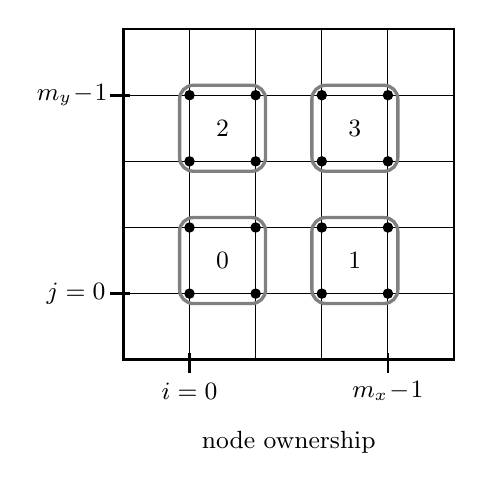
\begin{tikzpicture}[scale=4.2]
\gridsansowners
\pgfmathsetmacro\half{0.5*\fifth}
\pgfmathsetmacro\AA{0.15*\fifth}
\foreach \x in {1,3} {
    \foreach \y in {1,3} {
        \draw[very thick,rounded corners=5pt,gray] (\x*\fifth-\AA,\y*\fifth-\AA) -- (\x*\fifth+\fifth+\AA,\y*\fifth-\AA) -- (\x*\fifth+\fifth+\AA,\y*\fifth+\fifth+\AA) -- (\x*\fifth-\AA,\y*\fifth+\fifth+\AA) -- cycle;
    }
}
\node at (\fifth+\half,\fifth+\half) {\small $0$};
\node at (3*\fifth+\half,\fifth+\half) {\small $1$};
\node at (\fifth+\half,3*\fifth+\half) {\small $2$};
\node at (3*\fifth+\half,3*\fifth+\half) {\small $3$};
\node at (0.5,-0.25) {\small node ownership};
\end{tikzpicture}
\quad
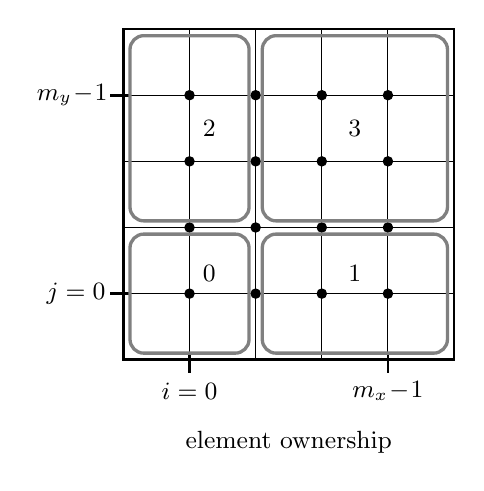
\begin{tikzpicture}[scale=4.2]
\gridsansowners
\pgfmathsetmacro\half{0.5*\fifth}
\pgfmathsetmacro\bit{0.3*\fifth}
\pgfmathsetmacro\BB{0.1*\fifth}
\draw[very thick,rounded corners=5pt,gray] (\BB,\BB) -- (2*\fifth-\BB,\BB) -- (2*\fifth-\BB,2*\fifth-\BB) -- (\BB,2*\fifth-\BB) -- cycle;
\draw[very thick,rounded corners=5pt,gray] (2*\fifth+\BB,\BB) -- (5*\fifth-\BB,\BB) -- (5*\fifth-\BB,2*\fifth-\BB) -- (2*\fifth+\BB,2*\fifth-\BB) -- cycle;
\draw[very thick,rounded corners=5pt,gray] (\BB,2*\fifth+\BB) -- (2*\fifth-\BB,2*\fifth+\BB) -- (2*\fifth-\BB,5*\fifth-\BB) -- (\BB,5*\fifth-\BB) -- cycle;
\draw[very thick,rounded corners=5pt,gray] (2*\fifth+\BB,2*\fifth+\BB) -- (5*\fifth-\BB,2*\fifth+\BB) -- (5*\fifth-\BB,5*\fifth-\BB) -- (2*\fifth+\BB,5*\fifth-\BB) -- cycle;
\node at (\fifth+\bit,\fifth+\bit) {\small $0$};
\node at (3*\fifth+\half,\fifth+\bit) {\small $1$};
\node at (\fifth+\bit,3*\fifth+\half) {\small $2$};
\node at (3*\fifth+\half,3*\fifth+\half) {\small $3$};
\node at (0.5,-0.25) {\small element ownership};
\end{tikzpicture}


\caption{Parallel distribution of interior nodes (left) and elements (right) in a $m_x=4$, $m_y=4$ grid.  Here there are four processes with ranks $0,1,2,3$.}
\label{fig:of:parallelgrid}
\end{figure}

Our scheme implies a slight load imbalance in the sense that ranks along the upper and right-hand side of the grid do more work.  This imbalance is quite tolerable if each rank owns a significant block of nodes, e.g.~a squarish block of thousands of interior nodes.

The main part, Code \ref{code:plapMain}, calls the various functions in the previous parts, of course.  We set up \pDMDA, some \pVecs, and \pSNES objects.  We use \texttt{DMCreateGlobalVector()} on \texttt{u} and \texttt{uexact}, but \texttt{DMCreateLocalVector()} on the \pVecs which hold $f$ and $g$.\sidenote{The latter \pVecs do not change during the run, so note that we never need to call \texttt{DMGlobalToLocalBegin/End()}.}  Also, we tell the \pSNES to use objective function \texttt{FormObjectiveLocal()} by calling
\begin{code}
    DMDASNESSetObjectiveLocal(da,(DMDASNESObjective)FormObjectiveLocal,&user);
\end{code}
which casts the type of \texttt{FormObjectiveLocal()} to the correct type for the call-back.\sidenote{\PETSc design choices require us to tell the \pDMDA that the \pSNES should use this objective function \dots}  Similarly, we call \texttt{DMDASNESSetFunctionLocal()} to tell the \pDMDA about \texttt{FormFunctionLocal()}; see Code \ref{code:plapFun} for the implementation.  Then we call \texttt{SNESSolve()}, compute the error, and destroy all the objects at the end.\sidenote{Regarding that last \texttt{Destroy()} step, the reader should check that it has no memory leaks once the program is built: \texttt{valgrind ./plap}}

These parts show the complete objective-only implementation.  To use it requires option \texttt{-snes\_fd\_function}, which does finite differencing on the objective functional $I^h[u]$, equation \eqref{eq:of:quadraturesumoverelements}, to get its gradient $\grad I^h[u]$.  Then the \pSNES solves the corresponding nonlinear system, $\bF(\bu) = \grad I^h[\bu] = 0$ in the notation of Chapter \ref{chap:nl}.

\cinputpart{plap.c}{\CODELOC}{In \texttt{main()} we set up \pDMDA, some \pVecs, and the \pSNES.  Then we solve and compute the error.}{VII}{//STARTMAIN}{//ENDMAIN}{code:plapMain}

However, even with a residual function $\bF(\bu)$ approximated this way, we still need a Jacobian for Newton's method.  To get that we ask \PETSc to finite difference \emph{again}, using either \texttt{-snes\_fd} or \texttt{-snes\_mf}.  For example:
\begin{cline}
$ cd c/ch6/
$ make plap
...
$ ./plap -snes_fd_function -snes_fd
grid of 3 x 3 = 9 interior nodes (element dims 0.25x0.25)
numerical error:  |u-u_exact|/|u_exact| = 8.081e-03
\end{cline}
%$

Recall from Chapter \ref{chap:nl} that we can ask \PETSc to count C function evaluations, to confirm that only the objective function is evaluated:
\begin{cline}
$ ./plap -snes_fd_function -snes_fd -log_view | grep Eval
SNESObjectiveEval    2198 1.0 1.8496e-01 1.0 ...
SNESJacobianEval       7 1.0 2.1275e-01 1.0 ...
\end{cline}
%$
No counts of ``\texttt{SNESFunctionEval}'' evaluations appear.  (The Jacobian evaluation counts report calls to \PETSc's finite difference Jacobian method.)  On the default grid of $3\times 3=9$ interior nodes grid we have evaluated the objective functional 2198 times!

However, experience from Chapter \ref{chap:nl} suggests using a ``coloring'' method, available for our \pDMDA-managed structured grid.  This reduces the evaluation count, here on a once-refined $5 \times 5$ grid:
\begin{cline}
$ ./plap -snes_fd_function -snes_fd -da_refine 1 -log_view | grep ObjectiveEval
SNESObjectiveEval   20539 1.0 1.5497e+00 1.0 ...
$ ./plap -snes_fd_function -snes_fd_color -da_refine 1 -log_view | grep ObjectiveEval
SNESObjectiveEval    5410 1.0 4.8340e-01 1.0 ...
\end{cline}
\label{page:of:badEvalcount}
Though better, this remains a disturbingly-large evaluation count.  These counts should be taken as a blunt warning that the method will not scale to fine grids.

Nonetheless, given that we have an implementation with an exact solution, we want to see convergence:\sidenote{Recall the \texttt{alias} \texttt{timer='time -f "real \%e"'} (Chapter \ref{chap:ls}).  This timing run is done with a ``\texttt{--with-debugging=0}'' configuration, a change of \texttt{PETSC\_ARCH}.}
\begin{cline}
$ for LEV in 0 1 2 3; do
> timer ./plap -snes_fd_color -snes_fd_function \
>   -snes_converged_reason -da_refine $LEV; done
grid of 3 x 3 = 9 interior nodes (element dims 0.25x0.25)
Nonlinear solve converged due to CONVERGED_FNORM_ABS iterations 6
numerical error:  |u-u_exact|/|u_exact| = 8.081e-03
real 0.05
grid of 5 x 5 = 25 interior nodes (element dims 0.166667x0.166667)
Nonlinear solve converged due to CONVERGED_FNORM_ABS iterations 7
numerical error:  |u-u_exact|/|u_exact| = 2.929e-03
real 0.10
grid of 9 x 9 = 81 interior nodes (element dims 0.1x0.1)
Nonlinear solve did not converge due to DIVERGED_LINEAR_SOLVE iterations 8
numerical error:  |u-u_exact|/|u_exact| = 9.253e-04
real 0.63
grid of 17 x 17 = 289 interior nodes (element dims 0.0555556x0.0555556)
Nonlinear solve did not converge due to DIVERGED_LINE_SEARCH iterations 20
numerical error:  |u-u_exact|/|u_exact| = 2.582e-04
real 16.48
\end{cline}
%$
This is evidence of convergence, with reductions of the error by factors close to $O(\Delta x^2)$.  However, on the two finer grids we get divergence of either the iterative linear solver (\texttt{DIVERGED\_LINEAR\_SOLVE}) or the Newton iteration (\texttt{DIVERGED\_LINE\_SEARCH}).  Such troubles are unsurprising when we observe that the Jacobian here is computed by finite-differencing a gradient computed by finite differences.\sidenote{Thank goodness we have 64 bit \texttt{double} precision, to get even this far.}  The Newton steps computed this way are too ``noisy.''

Taking stock and summarizing our situation, this prototype FEM method has allowed us to numerically-solve the $p$-Laplacian PDE in 2D by using \PETSc's ability to minimize a function.  Though performance is terrible, because of excessive objective evaluation, this capability can be a first step toward an effective code, and it can help with checking the correctness of better approaches.  We now try the most obvious ``better approach,'' namely computing the gradient of $I^h[u]$.


\section{Residual function (gradient) implementation}

The clear limitations of the objective-only implementation are that grids other than the coarsest lead to unreasonable numbers of evaluations of the objective function, and that the finite-differenced gradient and Jacobian have low quality.  This is one way of explaining why the weak form of the $p$-Laplacian, equation \eqref{eq:of:plapweakform}, is the traditional starting point for describing an FEM.  We should, therefore, implement the weak form as the residual function ``$\bF(\bx)$'' needed for Newton's method.

Equation \eqref{eq:of:plapweakform} says $\grad I[u](v) = 0$ for all $v\in W_0^{1,p}(\Omega)$.  The corresponding statement for $u\in S_g^h$, and where $v$ is equal to a hat function---see Figure \ref{fig:of:q1hat} and recall such functions form a basis of $S_0^h$---will be one equation in the nonlinear system we solve.

Thus we require $u\in S_g^h$ to satisfy \eqref{eq:of:plapweakform} for each $v=\psi_{pq}$ corresponding to one of the $N$ interior nodes:
\begin{equation}
\int_\Omega |\grad u|^{p-2} \grad u \cdot \grad \psi_{pq} - f \psi_{pq} = 0, \label{eq:of:weakformbasis}
\end{equation}
for $p=0,\dots,m_x-1$ and $q=0,\dots,m_y-1$.  Again this integral can be expanded as a sum over elements,
\begin{equation}
\sum_{i=0}^{m_x} \sum_{j=0}^{m_y} \int_{\square_{ij}} |\grad u|^{p-2} \grad u \cdot \grad \psi_{pq} - f \psi_{pq} = 0 \label{eq:of:residualsumoverelements}
\end{equation}

\cinputpart{plap.c}{\CODELOC}{The residual function $\bF(\bu)$ corresponding to the weak form \eqref{eq:of:plapweakform}.  These two C functions implement \eqref{eq:of:weakformintegrandref} and \eqref{eq:of:residualcontributions}, respectively.}{VIII}{//STARTFUNCTION}{//ENDFUNCTION}{code:plapFun}

However, only four distinct hat functions $\psi_{pq}$ contribute to the integral over $\square_{ij}$.  They correspond to the element corners indexed by $\ell=0,1,2,3$; recall equation \eqref{eq:of:psionref}.  Therefore we define
\begin{equation}
H_{ij}^\ell(\xi,\eta) = \left[|\grad u|^{p-2} \grad u \cdot \grad \psi_{pq} - f \psi_{pq}\right]_{\square_\ast}, \label{eq:of:weakformintegrandref}
\end{equation}
where it is understood that the element reference map $\square_\ast \to \square_{ij}$ is in use and that $(p,q)$ is the global node index corresponding to local index $\ell$.  Also, ``$\grad$'' is in the $(x,y)$ variables, so chain rule \eqref{eq:of:gradpsionref} applies.  Further details are in Exercise \ref{chap:of}.\ref{exer:of:weakformintegrand}.

We do the element integrals in \eqref{eq:of:residualsumoverelements}, with integrand \eqref{eq:of:weakformintegrandref}, by using quadrature \eqref{eq:of:tensorgauss}.  That is, we construct a component of the residual, the one corresponding to the weak form and test function $\psi_{pq}$, by accumulating contributions from those elements $\square_{ij}$ where $\psi_{pq}$ has value one at the $\ell$th corner of element $\square_{ij}$:
\begin{equation}
F_{pq}(u) \mathrel{+}= \frac{h_x h_y}{4} \sum_{r=0}^{n-1} \sum_{s=0}^{n-1} w_r w_s H_{ij}^\ell(z_r,z_s).  \label{eq:of:residualcontributions}
\end{equation}
Formula \eqref{eq:of:residualcontributions} is implemented by \texttt{FormFunctionLocal()} in Code \ref{code:plapFun}.  Note that \texttt{FunIntegrand()} implements \eqref{eq:of:weakformintegrandref} by reusing tools from Code \ref{code:plapTool}.

There is one nonlinear equation $F_{pq}(u)=0$ for each of the $N$ interior nodes $(x_p,y_q)$.  Solving this nonlinear system of equations,
    $$\bF(\bu)=0,$$
as in Chapter \ref{chap:nl}, should determine all $N$ nodal values $u_{ij}$.

The new version using residual evaluation, without option \texttt{-snes\_fd\_function}, significantly accelerates the objective-only implementation.  Compare timing:\sidenote{Option \texttt{-snes\_fd\_function} only works as intended, i.e.~avoids use of the residual function, if one of \texttt{-snes\_fd} or \texttt{-snes\_fd\_color} is also present.  Compare Exercise \ref{chap:of}.\ref{exer:of:commentoutresidual}.}
\begin{cline}
$ timer ./plap -da_refine 3
...
real 0.06
$ timer ./plap -da_refine 3 -snes_fd_color -snes_fd_function
...
real 15.13
\end{cline}
Note that, because we are using a \pDMDA structured grid and we have \emph{not} provided a Jacobian through calling \texttt{DMDASNESSetJacobianLocal()}, the efficient ``coloring'' form of finite-differencing (\texttt{-snes\_fd\_color}) is the default method by which the \pSNES approximates a Jacobian.

The reason for the speed-up is that the function-evaluation counts are now reasonable.  For instance, consider the following run which does four Newton iterations on a grid with $N=25$ interior points:
\begin{cline}
$ ./plap -da_refine 1 -log_view | grep Eval
SNESFunctionEval      45 1.0 6.6156e-03 1.0 ...
SNESObjectiveEval       8 1.0 4.5586e-04 1.0 ...
SNESJacobianEval       4 1.0 6.4406e-03 1.0 ...
\end{cline}
%$
Compare the earlier \texttt{-snes\_fd\_function} result which generated thousands of objective evaluations.


\section{Convergence and quadrature}

We can now give convincing evidence that our implementation converges at the $O(h^2)$ rate expected from the theory of well-behaved\footnote{E.g.~on convex polygonal domains and with smooth coefficient functions.} uniformly-elliptic PDEs for such a $Q^1$ FEM \citep{Elmanetal2005}.  Running
\begin{cline}
$ for LEV in 0 1 2 3 4 5 6 7 8; do
> ./plap -snes_converged_reason -da_refine $LEV; done
\end{cline}
%$
generates the convergence result in Figure \ref{fig:of:plap-conv}.

\begin{figure}
\includegraphics[width=0.75\textwidth]{figs/plap-conv}
\caption{Convergence evidence for the $p=4$ case suggests \texttt{plap.c} correctly solves $p$-Laplacian equation \eqref{eq:of:plapweakform}.  Relative errors $\|u-u_{\text{exact}}\|_\infty / \|u_{\text{exact}}\|_\infty$ from the residual version (dots) coincide with the objective-only results (four coarsest grids only; circled).  Degree $n=1$ Gauss-Legendre quadrature (squares) generates systematically larger errors than the default $n=2$ degree results.}
\label{fig:of:plap-conv}
\end{figure}

Recall that we have implemented Gauss-Legendre quadrature in \texttt{plap.c} for degrees $n=1,2,3$, but so far we have only used the default $n=2$.  Now we can compare quadrature degrees and demonstrate a genuine performance/accuracy trade-off.  Because we are timing the runs we make two improvements:
\begin{itemize}
\item We use a \texttt{--with-debugging=0} \PETSc configuration.
\item Because the Jacobian is a positive-definite and symmetric,\sidenote{The Jacobian of a weak form from an optimization principle is symmetric.} we choose a preconditioned CG method (``\texttt{-ksp\_type cg -pc\_type icc}''; see Chapter \ref{chap:ls}).
\end{itemize}

Thus:
\begin{cline}
$ for N in 1 2 3; do timer ./plap -ksp_type cg -pc_type icc \
>   -snes_converged_reason -da_refine 6 -plap_quaddegree $N; done
grid of 129 x 129 = 16641 interior nodes (element dims 0.00769231x0.00769231)
Nonlinear solve converged due to CONVERGED_FNORM_RELATIVE iterations 11
numerical error:  |u-u_exact|/|u_exact| = 7.964e-06
real 1.66
grid of 129 x 129 = 16641 interior nodes (element dims 0.00769231x0.00769231)
Nonlinear solve converged due to CONVERGED_FNORM_RELATIVE iterations 11
numerical error:  |u-u_exact|/|u_exact| = 4.490e-06
real 4.45
grid of 129 x 129 = 16641 interior nodes (element dims 0.00769231x0.00769231)
Nonlinear solve converged due to CONVERGED_FNORM_RELATIVE iterations 11
numerical error:  |u-u_exact|/|u_exact| = 4.490e-06
real 8.76
\end{cline}
The conclusions are quite clear.  For our solving our $Q^1$ FEM equations:
\renewcommand{\labelenumi}{\emph{(\roman{enumi})}}
\begin{enumerate}
\item higher degree quadrature is more expensive than lower degree,
\item $n=2$ degree is the minimum needed for full accuracy.
\end{enumerate}

As shown in Figure \ref{fig:of:plap-conv}, there is a systematic reduction of accuracy using degree $n=1$ quadrature.  The $n=3$ errors are indistinquishable from $n=2$ results (not shown), but this is as expected \citep[subsection 1.4.2]{Elmanetal2005}.  There is no justification for using $n>2$ quadrature with our $Q^1$ FEM.
% FIXME: how much of the above is specific to the p=4 case?  what if p=2?  other p?

Examining the $n=1,2$ performance difference a bit more carefully, namely by adding option \texttt{-ksp\_converged\_reason} to the above options (not shown), we see that there are two opposing performance changes with $n=1$ quadrature.  On the one hand there are slightly more CG iterations with $n=1$.  On the other hand, the evaluation of the quadrature sum \eqref{eq:of:tensorgauss} in the $n=1$ case is so much faster that we still get twice the speed relative to the $n=2$ case.


\section{More about the Newton iteration}

We now dig a little deeper into the Newton iteration for our discretized $p$-Laplacian equation \eqref{eq:of:plapweakform}, considering parallel runs and dependence on the exponent $p$.  Before that, recall how to visualize the iteration via \PETSc's graphing command-line options.  One can examine the iterates $\bx_k$ or the Newton step $\bs$, respectively:
\begin{cline}
$ ./plap -da_refine 6 -snes_monitor -snes_monitor_solution draw -draw_pause 1
...
$ ./plap -da_refine 6 -snes_monitor -snes_monitor_solution_update draw -draw_pause 1
...
\end{cline}
The latter shows that near-boundary locations are the last ones to converge.

Compare the following runs, in serial and then on four processes:
\begin{cline}
$ ./plap -ksp_type cg -pc_type icc -snes_converged_reason -da_refine 6
grid of 129 x 129 = 16641 interior nodes (element dims 0.00769231x0.00769231)
Nonlinear solve converged due to CONVERGED_FNORM_RELATIVE iterations 11
numerical error:  |u-u_exact|/|u_exact| = 4.490e-06
$ mpiexec -n 4 ./plap -ksp_type cg -pc_type bjacobi -sub_pc_type icc -snes_converged_reason -da_refine 6
grid of 129 x 129 = 16641 interior nodes (element dims 0.00769231x0.00769231)
Nonlinear solve did not converge due to DIVERGED_LINE_SEARCH iterations 9
numerical error:  |u-u_exact|/|u_exact| = 2.859e-05
\end{cline}
The parallel run did not converge!  By a bit of trial-and-error\sidenote{E.g.~using \texttt{-snes\_monitor -ksp\_converged\_reason}.} one finds that coarser grids are sometimes o.k.~in parallel with these options, but this \texttt{DIVERGED\_LINE\_SEARCH} failure occurs on most grids.

The default ``back-tracking'' method has difficulties here, but apparently only in parallel.  Trying other line search methods (Table \ref{tab:nl:linesearchoptions}) resolves the issue.  Types \texttt{basic} and \texttt{cp}, the latter of which uses the objective function we provided instead of substituting a least-squares merit function (Chapter \ref{chap:nl}), both work just fine in parallel.  We also try now to get a fine grid solution.  The following run takes several minutes and converges:
\begin{cline}
$ timer mpiexec -n 4 ./plap -ksp_type cg -pc_type bjacobi -sub_pc_type icc \
>    -snes_converged_reason -da_refine 9 -snes_linesearch_type cp
grid of 1025 x 1025 = 1050625 interior nodes (element dims 0.000974659x0.000974659)
Nonlinear solve converged due to CONVERGED_FNORM_RELATIVE iterations 11
numerical error:  |u-u_exact|/|u_exact| = 1.493e-07
real 489.73
\end{cline}
%$
The good news is that everything works with $N=10^6$ degrees of freedom.  However, we are still exposed to the bad scaling, with respect to $N$, of the preconditioned CG method (Chapter \ref{chap:ls}).\sidenote{To illustrate this add option \texttt{-ksp\_converged\_reason}.}  In Chapter \ref{chap:pr} we will look at better preconditioning, and in Chapter \ref{chap:sc} larger processor-counts, for this same example.


\section{Dependence on the exponent $p$}

Convergence varies depending on the exponent $p$.  Recall that the Sobolev space $W^{1,p}(\Omega)$ and the objective functional $I[u]$---see equation \eqref{eq:of:functional}---are defined for any $1 \le p < \infty$, but that $I[u]$ is not continuously-differentiable when $p=1$.

We can investigate the way our problem actually depends on $p$ by \emph{measuring} the error for a sampling of $p$-values, as in this double loop for example:
\begin{cline}
$ for PP in 1.1 2.1 4 10; do
>   for LEV in 0 1 2 3 4 5 6 7 8; do
>     ./plap -snes_converged_reason -da_refine $LEV \
>            -ksp_type cg -pc_type icc -plap_p $PP;
>   done; done
\end{cline}
%$
This includes the $p=4$ results shown in Figure \ref{fig:of:plap-conv}, but also $p$ near the linear case and $p$ near the extremes: $p=1.1,10$.  Regarding exponent $p=2.1$, and speaking intuitively, the distance from $p$ to $p=2$ is a measure of the degree of nonlinearity.\sidenote{When $p=2$ the objective is quadratic and equation \eqref{eq:of:plapstrongform} is linear (in $u$).}  It is not surprising that the $p=2.1$ case has the smallest errors and the lowest number of Newton iterations.

\begin{figure}
\includegraphics[width=0.75\textwidth]{figs/plap-perrs}
\caption{Relative errors for $p=1.1,2.1,4,10$; compare Figure \ref{fig:of:plap-conv}.}
\label{fig:of:plap-perrs}
\end{figure}

The relative errors generated from our double loop are shown in Figure \ref{fig:of:plap-perrs}.  We see that $p = 1.1 \approx 1$ is not apparently as hard as a large value such as $p=10$.

For $p=10$ we have non-convergence on the finest grid---thus that case is not shown---but the Newton iteration converges in all other cases.  The fact that, when $p=10$, the measured error \emph{increases} as $h\to 0$ for the finest three grids is suspicious: the solution of the discrete nonlinear equations apparently diverges from the exact (continuum) solution.

The Newton iteration counts generated by the above double loop are shown in Figure \ref{fig:of:plap-piters}.  Again the $p=10$ case seems to be the most difficult.

We have seen that the nonlinearity for large $p$ seems to be more difficult than the cases near $p=1$, but how about $p=1$ itself?  The result of
\begin{cline}
for LEV in 0 1 2 3 4 5 6 7 8; do
>  ./plap -snes_converged_reason -da_refine $LEV \
>         -ksp_type cg -pc_type icc -plap_p 1; done
\end{cline}
%$
is that we get \texttt{DIVERGED\_LINEAR\_SOLVE} errors on the four finest grids (not shown).  One possible approach would be to change to a direct solver, in an attempt to resolve that error directly.  A different approach, coming from the idea that the underlying objective is not differentiable, is to regularize the problem by making the weak form more differentiable---see Exercise \ref{chap:of}.\ref{exer:of:regularizepone}.
\label{page:of:casepone}

\begin{figure}
\includegraphics[width=0.72\textwidth]{figs/plap-piters}
\caption{Newton iterations for $p=1.1,2.1,4,10$.}
\label{fig:of:plap-piters}
\end{figure}


\section{Condition number, ellipticity, and regularization}  \label{page:of:condellip}

The solution of the $p$-Laplacian equation so far in this Chapter is ``dangerous'' in that we have treated the equation as though it is a uniformly-elliptic linear PDE \citep{Evans2010}.  Such a statement is problem- and method-dependent for the $p$-Laplacian because of the solution-dependent coefficient $|\grad u|^{p-2}$ in both the weak \eqref{eq:of:plapweakform} and strong \eqref{eq:of:plapstrongform} forms.  Note that we do have bounds on the coefficient for the case of exact solution $u=u_{\text{exact}}$---see \eqref{eq:of:exactsolution} and Exercise \ref{chap:of}.\ref{exer:of:checkexactbounds}.  Namely, if $\alpha>0$ then
\begin{equation}
0 < 2^{(p-2)/2} \alpha^{3(p-2)} \le |\grad u|^{p-2} \le 2^{(p-2)/2} \left(1+\alpha\right)^{3(p-2)}.  \label{eq:of:coeffbounds}
\end{equation}

For other source terms $f$ or boundary conditions $g$, however, there might be no such bounds.  The Newton iterates could also make $|\grad u|^{p-2}$ much larger or smaller, in some parts of the domain, than its values at the solution.  On the practical side, coefficient bounds are a measure of uniform ellipticity which relates to the condition number of the discrete linear system.\sidenote{Recall that the condition number $\kappa(A)$ in equation \eqref{eq:ls:conddefn} describes the perturbation-sensitivity of the linear system.  It also controls the convergence of the CG iteration if $A$ is symmetric and positive-definite, as it is here.  See Chapter \ref{chap:ls}.}

One may ask \PETSc for an estimate of the condition number, that is, of the linear system solved at each Newton step, by option

\centerline{\texttt{-ksp\_compute\_singularvalues}}

\noindent The output then includes a line
\begin{code}
Iteratively computed extreme singular values: max X min Y max/min Z
\end{code}
for each Newton step.  Recalling that the 2-norm condition number $\kappa_2(A)=\sigma_{\text{max}}/\sigma_{\text{min}}$ is the ratio of the largest to smallest singular value of $A$ \citep{TrefethenBau1997}, here \texttt{Z = X/Y} is the estimated condition number.

However, an important consideration is that \PETSc generates the condition number of the \emph{preconditioned} linear system.\sidenote{E.g.~system \eqref{introleftpre} instead of system \eqref{introsystem}, in Chapter \ref{chap:ls}, under (default) left-preconditioning.}  For example, compare the results of
\begin{cline}
$ ./plap -pc_type cholesky -ksp_type cg -ksp_compute_singularvalues
$ ./plap -pc_type none -ksp_type cg -ksp_compute_singularvalues
\end{cline}
The former reports a condition number of 1 at the end of the iteration while the latter says it is about 10.75.  The former value merely says that the Cholesky direct solver generated an $M$ so that $M^{-1} A=I$, i.e.~$M^{-1}=A^{-1}$, and thus $\kappa_2(M^{-1} A)=1$.  This is the ``extreme preconditioner'' in which the linear system has become trivial.  The second of the above commands, with option \texttt{-pc\_type none}, instead gives the computed condition number $\kappa_2(A)$ for the unmodified Jacobian $A$; this is what we want.

How does this relate to ellipticity?  The theory of the errors of FE methods for linear, uniformly-elliptic, convex polygonal domain PDE problems says that discrete linear system condition numbers increase as the grid is refined.  Specifically,  \citet{Elmanetal2005} Theorem 1.32 shows
    $$\kappa_2(A) \le C h^{-2}$$
for a constant $C$ that relates implicitly to the (ellipticity) bounds on the coefficient of the operator.  This upper bound, whose derivation suggests that in fact $O(h^{-2})$ is the expected rate of growth, is one more reason why finer grid solutions are more difficult to compute than coarser grid solutions.

The $O(h^{-2})$ growth rate is roughly what we see here in practice, even though our equation is nonlinear.  For example, the loop
\begin{cline}
$ for LEV in 0 1 2 3 4 5 6; do
>   ./plap -pc_type none -ksp_type cg -ksp_rtol 1.0e-14 -da_refine $LEV \
>      -ksp_compute_singularvalues; done
\end{cline}
generates the lower curve in Figure \ref{fig:of:plap-conditionnumber}.

\begin{figure}
\includegraphics[width=0.95\textwidth]{figs/plap-conditionnumber}
\caption{The condition number $\kappa_2(A)$ of the linearized operator grows at about the expect $O(h^{-2})$ rate when $\alpha=1$ in exact solution \eqref{eq:of:exactsolution} (dots).  However, when $\alpha=0.1$ the practical effect is that the condition number is bigger and grows faster (squares).}
\label{fig:of:plap-conditionnumber}
\end{figure}

To illustrate that the condition number is related to bounds on the coefficient $|\grad u|^{p-2}$, first note that the parameter $\alpha$ in exact solution \eqref{eq:of:exactsolution} has, so far, been set to $\alpha = 1$.  However, if $\alpha=0$ then the exact solution is $u_{\text{exact}}(x,y) = \frac{1}{2} x^2 y^2$.  Now $\grad u \to 0$ as $(x,y)\to(0,0)$ in $\Omega$, so that $|\grad u|^{p-2}$ is not bounded-below by a positive constant on $\Omega$.

Before we can see the effect computationally, note that option \texttt{-plap\_alpha 0} does not work because the value of the source term at the lower-left corner, namely $f(0,0)$, is then undefined.\sidenote{See Exercise \ref{chap:of}.\ref{exer:of:checkexactformulas}.  To see the run-time effect, however, just try it.}  However, adding \texttt{-plap\_alpha 0.1} to the above Bash loop yields much larger condition numbers for the coarsest five grids, as shown in Figure \ref{fig:of:plap-conditionnumber}, while on the two finest grids we get \texttt{DIVERGED\_LINEAR\_SOLVE}.

In a bit more detail, when $\alpha=0.1$ the upper and lower bounds on the coefficient (see Exercise \ref{chap:of}.\ref{exer:of:checkexactbounds}), and the largest and smallest singular values, are \emph{all} smaller than in the $\alpha=1$ case.  But the lower bound on the coefficient, and the smallest singular value, are \emph{much} smaller than when $\alpha=1$.  As seen in Figure \ref{fig:of:plap-conditionnumber}, the result is that the condition number is orders of magnitude larger on finer grids.  Because it is so much harder for the coarse-grid problems to approximate the correct continuum values of the Newton steps $\bs$, the growth rate of the condition number, as $h$ decreases through a sequence of relatively-coarse grids, is much faster than $O(h^{-2})$.  This effect is seen in Figure \ref{fig:of:plap-conditionnumber}.  The condition number growth then seems to ``level-out'' as the grids become finer, and presumably $O(h^{-2})$ is achieved for sufficiently small $h$-values.

On a somewhat-fine grid we can get converged runs with $\alpha=0.1$ if we do not ask for full accuracy in solving the linear system:
\begin{cline}
$ ./plap -ksp_type cg -pc_type none -da_refine 5 \
>     -ksp_compute_singularvalues -snes_converged_reason -plap_alpha 0.1
grid of 65 x 65 = 4225 interior nodes (element dims 0.0151515x0.0151515)
...
Iteratively computed extreme singular values: max 22.1875 min 7.68515e-06 max/min 2.88706e+06
Nonlinear solve converged due to CONVERGED_FNORM_RELATIVE iterations 11
numerical error:  |u-u_exact|/|u_exact| = 1.988e-04
\end{cline}
%$
(The default tolerance used here is \texttt{ksp\_rtol 1.0e-5}.)  For comparison to results below, note the estimated condition number $\kappa(A)=2.9\times 10^6$ is quite large, and that the numerical error is about $2.0\times 10^{-4}$.

Can the condition number be improved?  One common approach is to \emph{regularize} the $p$-Laplacian by inserting a constant $\eps>0$ so that the weak form \eqref{eq:of:plapweakform} becomes
\begin{equation}
\int_\Omega \left(|\grad u|^2+\eps^2\right)^{(p-2)/2} \grad u \cdot \grad v - f v = 0. \label{eq:of:plapweakformreg}
\end{equation}
Thus a positive lower bound on the coefficient is guaranteed,
     $$0 < \eps^{p-2} \le \left(|\grad u|^2+\eps^2\right)^{(p-2)/2},$$
so that if we linearize the problem around any $u\in W^{1,p}(\Omega)$ then the resulting linear, weak-form PDE is uniformly-elliptic.

This regularization is already implemented in \texttt{plap.c}, but the default $\eps=0$ has been used in all runs so far.  Here we can demonstrate that regularization works in at least one case:
\begin{cline}
$ ./plap -ksp_type cg -pc_type none -da_refine 5 \
>     -ksp_compute_singularvalues -snes_converged_reason \
>     -plap_alpha 0.1 -plap_eps 0.01
grid of 65 x 65 = 4225 interior nodes (element dims 0.0151515x0.0151515)
...
Iteratively computed extreme singular values: max 22.1876 min 3.44109e-05 max/min 644783.
Nonlinear solve converged due to CONVERGED_FNORM_RELATIVE iterations 11
numerical error:  |u-u_exact|/|u_exact| = 1.305e-04
\end{cline}
%$
That is, adding $\eps=0.01$ to the previous run gives \emph{both} a lower estimated condition number \emph{and} a lower error.

Such a result is not at all automatic!  As the reader can confirm through experimentation,  we have ``cherry-picked'' an example to demonstrate this result.  The user can experiment with the effect of regularization (\texttt{-plap\_eps}), across a range of nonlinearities (\texttt{-plap\_p}) and exact solutions\sidenote{Observe that adjusting $\alpha$ controls the exact solution \emph{and} the uniform-ellipticity bounds at the solution.} \texttt{-plap\_alpha}, and thereby form an observation-based opinion of the effectiveness of it. 

We will see in Chapter \ref{chap:co} that, in certain problems which are related to the $p$-Laplacian, namely the ice sheet flow model shown in that Chapter, a loss of ellipticity (``degeneracy'') is physically-meaningful.  In such cases we introduce additional information into the problem (i.e.~inequality constraints), as well as a modified Newton solver from \PETSc, so as to get higher-quality solutions with minimal regularization.


\section{Summary}

The $p$-Laplacian problem in this Chapter has been used to explore a number of ideas:
\begin{itemize}
\item the connection between optimization problems and PDEs,
\item the implementation of structured-grid $Q^1$ finite element method,
\item the effect of varying quadrature degree in an FEM,
\item options for the Newton-Krylov method, and
\item convergence issues for a non-linear elliptic problem.
\end{itemize}

Only modest success comes from our initial objective-only implementation, but it is a usable prototyping tool with a ``side-effect'', in this case, of providing \PETSc's line search with the right objective.  Then, once we add the traditional residual-evaluation function, we achieve substantial success, on relatively-high-resolution grids, without an analytical Jacobian.

We will return to look at performance of this example in Chapter \ref{chap:sc}, and, as already noted, to a related problem in Chapter \ref{chap:co}.


\section{Exercises}

\renewcommand{\labelenumi}{\arabic{chapter}.\arabic{enumi}\quad}
\renewcommand{\labelenumii}{(\alph{enumii})}
\begin{enumerate}
\item  \label{exer:of:twoproperties}  \emph{This two-part exercise is a mathematical excursion which some readers may wish to skip.}
  \begin{enumerate}
  \item For $1 \le p < \infty$, prove coercivity \eqref{eq:of:coercivity} of functional $I[u]$, defined in \eqref{eq:of:functional}, on $W_0^{1,p}(\Omega)$.  (\emph{Hints}:  Use Poincar\`e inequality \citep[Theorem 6.30]{AdamsFournier2003} to replace the leading term with the full $W^{1,p}$ norm.  Use Young's inequality with $\epsilon>0$ \citep[Appendix B]{Evans2010} for the ``$-fu$'' term.  Now choose $\eps$ appropriately.)
  \item For $1 < p < \infty$, prove strict convexity \eqref{eq:of:convexity} of functional $I[u]$ on $W_0^{1,p}(\Omega)$.  (\emph{Hint}:  The argument in section 5.3 of \citet{Ciarlet2002} suffices.)
  \end{enumerate}
 
\item \label{exer:of:checkexactformulas}  For the exact solution $u=u_{\text{exact}}$ in \eqref{eq:of:exactsolution}, define $C = |\grad u|^{p-2}$ and $D^2=(x+\alpha)^2 + (y+\alpha)^2$.  Show that
    $$C = \left[(x+\alpha)^2 (y+\alpha)^2 D^2\right]^{(p-2)/2}$$
and that $\grad C = (p-2) C \left<\gamma_1,\gamma_2\right>$ where
    $$\gamma_1 = \frac{1}{x+\alpha}+ \frac{x+\alpha}{D^2}, \quad \gamma_2 = \frac{1}{y+\alpha}+ \frac{y+\alpha}{D^2}.$$
Also show that $\Div \grad u = D^2$.  Thus strong form \eqref{eq:of:plapstrongform} implies the following formula for the source function:
    $$f = - \Div \left(C \grad u\right) = - \grad C \cdot \grad u - C\, \Div \grad u.$$
Check that \texttt{ExactRHSLocal()} in \texttt{plap.c} implements these formulas.

\item \label{exer:of:checkexactbounds}  For the exact solution $u=u_{\text{exact}}$ in \eqref{eq:of:exactsolution}, show that if $\alpha>0$ then \eqref{eq:of:coeffbounds} holds.  Also show that if $-1 \le \alpha \le 0$ then there is a point in $\bar\Omega=[0,1]\times[0,1]$ so that $|\grad u|^{p-2}=0$.

\item Show that $S^h$ is a linear subspace of $W^{1,p}(\Omega)$ with dimension $(m_x+2)(m_y+2)$, and that $S_0^h$ has dimension $m_x m_y$.  What precisely is meant by saying $g$ is ``(appropriately) piece-wise linear on $\partial\Omega$'' in the definition of $S_g^h$ on page \pageref{eq:of:Sghdefn}?  Is our use of exact solution \eqref{eq:of:exactsolution} to give $g$ ``appropriate'' in this sense?

\item  Use \eqref{eq:of:refcorners} and \eqref{eq:of:chidefn} to show that the two forms of the reference map \eqref{eq:of:referencemap} are the same.  Then use \eqref{eq:of:chidefn}, \eqref{eq:of:referencemap}, and \eqref{eq:of:psionref} to derive \eqref{eq:of:gradpsionref}.

\item By testing against the integral
    $$\int_{\square_\ast} (1+\xi)^k + (1+\eta)^k\,d\xi\, d\eta = \frac{2^{k+3}}{k+1}$$
for $k=0,1,\dots,6$, confirm that the $n=1,2,3$ Gauss-Legendre quadrature formulas listed in the text will exactly integrate degree $2n-1$ degree polynomials, but not degree $2n$ polynomials, on the reference element.  (\emph{Use the computer language of your choice.})
% solution:  matlab/testgauss2d.m

\item \label{exer:of:integrand}  Show that \eqref{eq:of:integrandheuristic} is, in detail,
\begin{align*}
G_{ij}(\xi,\eta) &= \frac{1}{p} \left[\frac{4}{h_x^2} \left(\sum_{\ell=0}^3 u_\ell \frac{\partial\chi_\ell}{\partial \xi}\right)^2 + \frac{4}{h_y^2} \left(\sum_{\ell=0}^3 u_\ell \frac{\partial\chi_\ell}{\partial \eta}\right)^2\right]^{p/2} \\
  &\qquad - \left(\sum_{\ell=0}^3 f_\ell \chi_\ell\right) \left(\sum_{\ell=0}^3 u_\ell \chi_\ell\right)
\end{align*}
where $u_\ell$ and $f_\ell$ are local-node-numbered values of $u$ and $f$ on element $\square_{ij}$.

\item \label{exer:of:weakformintegrand}  Show that for local node index $L=0,1,2,3$, \eqref{eq:of:weakformintegrandref} is, in detail,
\begin{align*}
H_{ij}^L(\xi,\eta) &= \left[\frac{4}{h_x^2} \left(\sum_{\ell=0}^3 u_\ell \frac{\partial\chi_\ell}{\partial \xi}\right)^2 + \frac{4}{h_y^2} \left(\sum_{\ell=0}^3 u_\ell \frac{\partial\chi_\ell}{\partial \eta}\right)^2\right]^{(p-2)/2} \\
  &\qquad \cdot \left[\frac{4}{h_x^2} \left(\sum_{\ell=0}^3 u_\ell \frac{\partial\chi_\ell}{\partial \xi}\right) \frac{\partial\chi_L}{\partial \xi} + \frac{4}{h_y^2} \left(\sum_{\ell=0}^3 u_\ell \frac{\partial\chi_\ell}{\partial \eta}\right) \frac{\partial\chi_L}{\partial \eta}\right] \\
  &\quad - \left(\sum_{\ell=0}^3 f_\ell \chi_\ell\right) \chi_L.
\end{align*}

\item Figure \ref{fig:of:cartoonfunctional} shows the graph of $\Phi(x,y)=\tfrac{1}{4}(x^4+y^4) - 2x + 2y$, a cartoon for the $p$-Laplacian functional $I[u]$ in the case $p=4$.  Solve
    $$\min_{x,y} \Phi(x,y)$$
by hand.  Now write a \PETSc code \texttt{cartoon.c} to solve this problem, starting with a code that only implements $\Phi(x,y)$ by a function \texttt{FormObjective()} and a call to \texttt{SNESSetObjective()}.  After checking that it works using ``\texttt{./cartoon -snes\_fd\_function -snes\_fd},'' add a function \texttt{FormFunction()} and a call to \texttt{SNESSetFunction()} and check that now ``\texttt{./cartoon -snes\_fd}'' works.

\emph{Hints}.  Note that your code will \emph{not} use a \pDMDA, because there is no underlying grid (or differential equation).  Consider \texttt{expcircle.c} from Chapter \ref{chap:nl} as a starting point for your code.
% solution:  c/\CODELOC solns/cartoon.c

\item \label{exer:of:commentoutresidual}  Comment-out those parts of \texttt{plap.c} which are shown in Code \ref{code:plapFun}, and the \texttt{DMDASNESSetFunctionLocal()} line shown in Code \ref{code:plapMain}.  Thus you have removed all references to \texttt{FormFunctionLocal()}, so you have a truly ``objective-only'' code.  Confirm that
\begin{cline}
./plap -snes_fd_color -snes_fd_function
\end{cline}
still works, but that ``\texttt{./plap -snes\_fd}'' and ``\texttt{./plap -snes\_mf}'' do not.  Confirm the evaluation-counting results in the main text which use ``\texttt{-log\_view | grep Eval}'' on the objective-only implementation.

\item \label{exer:of:regularizepone}  The $p=1$ cases tried on page \pageref{page:of:casepone} are problematic because, in terms of the minimization of $I[u]$,  we are applying a gradient-based method to minimize a non-smooth \citep{NocedalWright2006} functional.  One might suppose that the regularized weak form \eqref{eq:of:plapweakformreg}, which is smooth for $\eps>0$, should work better, but this hypothesis needs testing.  Add option \texttt{-plap\_eps} $\eps$,\sidenote{And possibly option \texttt{-snes\_max\_it 200} if needed.} to the $p=1$ Bash loop shown on page \pageref{page:of:casepone}.  Try various values of regularization parameter $\eps>0$.  Is regularization effective for resolving \emph{this} non-smooth problem?

\item Especially with $\alpha=0.1$, so that the problem is less uniformly-elliptic, the norm we use in evaluating the relative error $\|u-u_{exact}\|/\|u_{exact}\|$ makes a difference to the observed convergence rate.  Add an option to \texttt{plap.c} to choose either the $\infty$-norm or the 1-norm.  Regenerate the main data (i.e.~the dots) Figure \ref{fig:of:plap-conv} in the case $\alpha=0.1$ and using the 1-norm, and recompute the convergence rate $q$ in ``$O(h^q)$''.  What does 1-norm convergence measure?

\item One may approximate the strong form PDE \eqref{eq:of:plapstrongform} by finite differences using essentially the same structured grid as in this Chapter.  However, note that in Chapter \ref{chap:st} we treated the boundary values as unknowns, but with trivial equations.  This can be done for \eqref{eq:of:plapstrongform} too.  Construct such a finite-difference, \pSNES- and \pDMDA-using program \texttt{plapfd.c}.  It should implement the residual function, but, at least initially, there is no need to implement the objective or the Jacobian---compare Exercises \ref{chap:of}.\ref{exer:of:picardimplementation} and \ref{chap:of}.\ref{exer:of:jacobianimplementation} below.  Use the same manufactured solution \eqref{eq:of:exactsolution} as here.  Compare convergence and performance.  Summarize differences, including ease-of-implementation, in a few sentences.

\item  Though we did not mention or show it, the runs in this Chapter generally demonstrate quadratic convergence of the Newton iteration.  Show the evidence for this claim by making a figure, like Figure \ref{fig:newtonconvbasic}, for the runs which are shown as dots in Figure \ref{fig:of:plap-conv}.

\item \label{exer:of:picardimplementation}  It is common to linearize the strong form PDE \eqref{eq:of:plapstrongform} as a \emph{Picard} iteration, either to reuse linear-problem tools, or to avoid implementing a Jacobian.  Let $u^{(k)}$ be the $k$th step of this iteration.  Given the earlier iterate $u^{(k-1)}$, we solve
\begin{equation}
- \Div\left(|\grad u^{(k-1)}|^{p-2} \grad u^{(k)}\right) = f.
\label{eq:of:picard}
\end{equation}
Implement this method by adding a function \texttt{FormPicardLocal()} to \texttt{plap.c}.  This function computes and assembles a \pMat for the left side, so that \eqref{eq:of:picard} is a linear equation $A\bu = \bb$ at each iteration.  Use \texttt{MatSetValuesStencil()} to insert entries into the \pMat; how many nonzero entries are there per row?  Also add this line to \texttt{main()}:
\begin{code}
    DMDASNESSetJacobianLocal(user.da,
            (DMDASNESJacobian)FormPicardLocal,&user);
\end{code}
Run the code and check using \texttt{-log\_view | grep Eval} that the number of evaluations of \texttt{FormFunctionLocal()} is much smaller than before.  Recover quadratic convergence with option \texttt{-snes\_mf\_operator}, which uses the Picard matrix as preconditioner ``material'' (Chapter \ref{chap:nl}).

\item \label{exer:of:jacobianimplementation}  Improve on the last exercise by implementing the true Jacobian.  Add a user option so that either the Picard or Jacobian matrix is used, and compare performance with: the true Jacobian, the Picard matrix used as the true Jacobian, and the Picard matrix used with option \texttt{-snes\_mf\_operator}.

\end{enumerate}

